%=========================================================================
% (c) 2014, 2015 Josef Lusticky

\subsection{Traffic generation}
The RFC~2544 specifies the following frame sizes to be used on Ethernet:
64, 128, 256, 512, 1024, 1280 and 1518~\cite{rfc2544}.
However, at least 66~B frame size must be used in case of transmitting UDP over IPv6 - the size of L2 header is 14,
the size of CRC is 4, the size of IPv6 header is 40 and the size of UDP header is 8.

In addition to the specified frame sizes, a custom frame size distribution can be defined for the purpose of
a real internet traffic simulation.
The Amsterdam Internet Exchange (AMS-IX) provides
statistics of the frame size distribution in the Internet traffic~\cite{amsix-frame-size}.
Figure~\ref{fig:analysis-amsix-frame-size} shows yearly frame size distribution provided by AMS-IX.
This distribution can be configured in the Spirent TestCenter Application, however,
to use the same iMix for both IPv4 and IPv6, the minimum frame size must be increased to 66 as described above.
To avoid an unfair packet scheduling by the server, all packets should be assigned the same Type of Service flag.

\begin{figure}
	\centering
	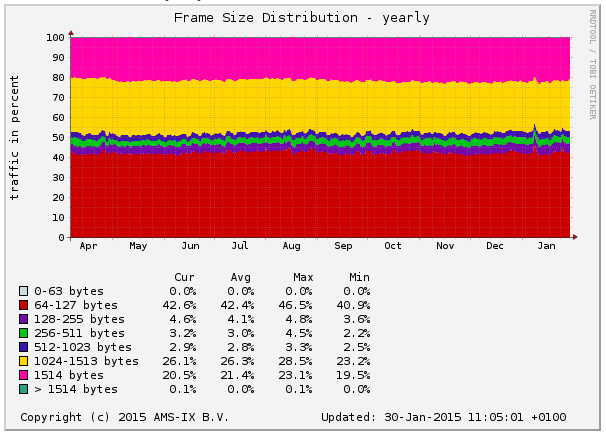
\includegraphics[width=14.5cm,keepaspectratio]{fig/amsix.png}
	\caption{Yearly frame size distribution at AMS-IX (source:~\cite{amsix-frame-size})}
	\label{fig:analysis-amsix-frame-size}
\end{figure}
